
\chapter{Architecture}

\section{Tokenization}

\subsection{Logic}

\paragraph{UTF-8} 
The MSMARCO corpus contains several wrongly encoded documents, it seems their \textit{spider} wrongly interpreted certain documents as encoded in \texttt{latin1} --- a eight bit ASCII extension used by old Microsoft's software --- instead of \texttt{UTF-8} and then converted them in \texttt{UTF-8} interpreting their bytes as \texttt{UTF-8} data. To solve this issue we wrote a simple heuristic that tries to detect strange Unicode's entry-points that are likely the result of the processes; and a reverse encoding procedure that converts them back in their original \texttt{UTF-8} form. We didn't perform experiments so we cannot tell if this actually improves accuracy on the testing corpus.

\paragraph{Punctuation and splitting}
Our implementation takes a very simplistic approach to punctuation handling, that is all known western punctuation is removed and replaced with spaces, you can see the punctuation handled by the program in the source file \texttt{normalizer/PunctuationRemover.cpp}.

Words, that are tokens, are generated by splitting the resulting text by spaces.

\paragraph{Lower case}
Changing case of a Unicode word is a non trivial task and there are no fast ready-to-use libraries that directly operate on \texttt{UTF-8} --- instead they require a conversion to \texttt{UTF-16} or \texttt{UTF-32}, that we'd rather avoid, --- nevertheless we decided not to limit ourselves to only handle the case of ASCII's latin letters but we convert the case of \textit{latin1}'s latin letters --- that is a larger subset of Unicode latin letters. In conclusion most words written in latin characters are converted in lower-case.

\paragraph{Stemming}
Stemming is done using the Porter algorithm.

\subsection{Libraries}

\paragraph{Punctuation}
To replace punctuation with spaces we make use of regex expressions and run them on Hyperscan (or Vectorscan on non amd64 platforms), that is a fast regex engine that make use of SIMD instructions --- such as AVX-512 --- to speed up their solution.

\paragraph{Stemming}
To stem words, we make of the famous Snowball's stemmer implementation.

\section{Indices' organization}

\paragraph{}
We've designed the system to partition by document, that is we divide the entire document collection in multiple sub-collections, making it possible to parallelize the query execution on multiple machines in a \textit{computing cluster} or on a multi-disk single machine or both.

\paragraph{MapReduce}
We can think of the query solution problem as a map-reduce problem, as illustrated in Figure \ref{fig:mapreduce}; that is each partition runs on a separated process that generates the top-$k$ documents for its own data, finally a merger procedure generates the global top-$k$ results.

\begin{figure}[h]
	\centering
	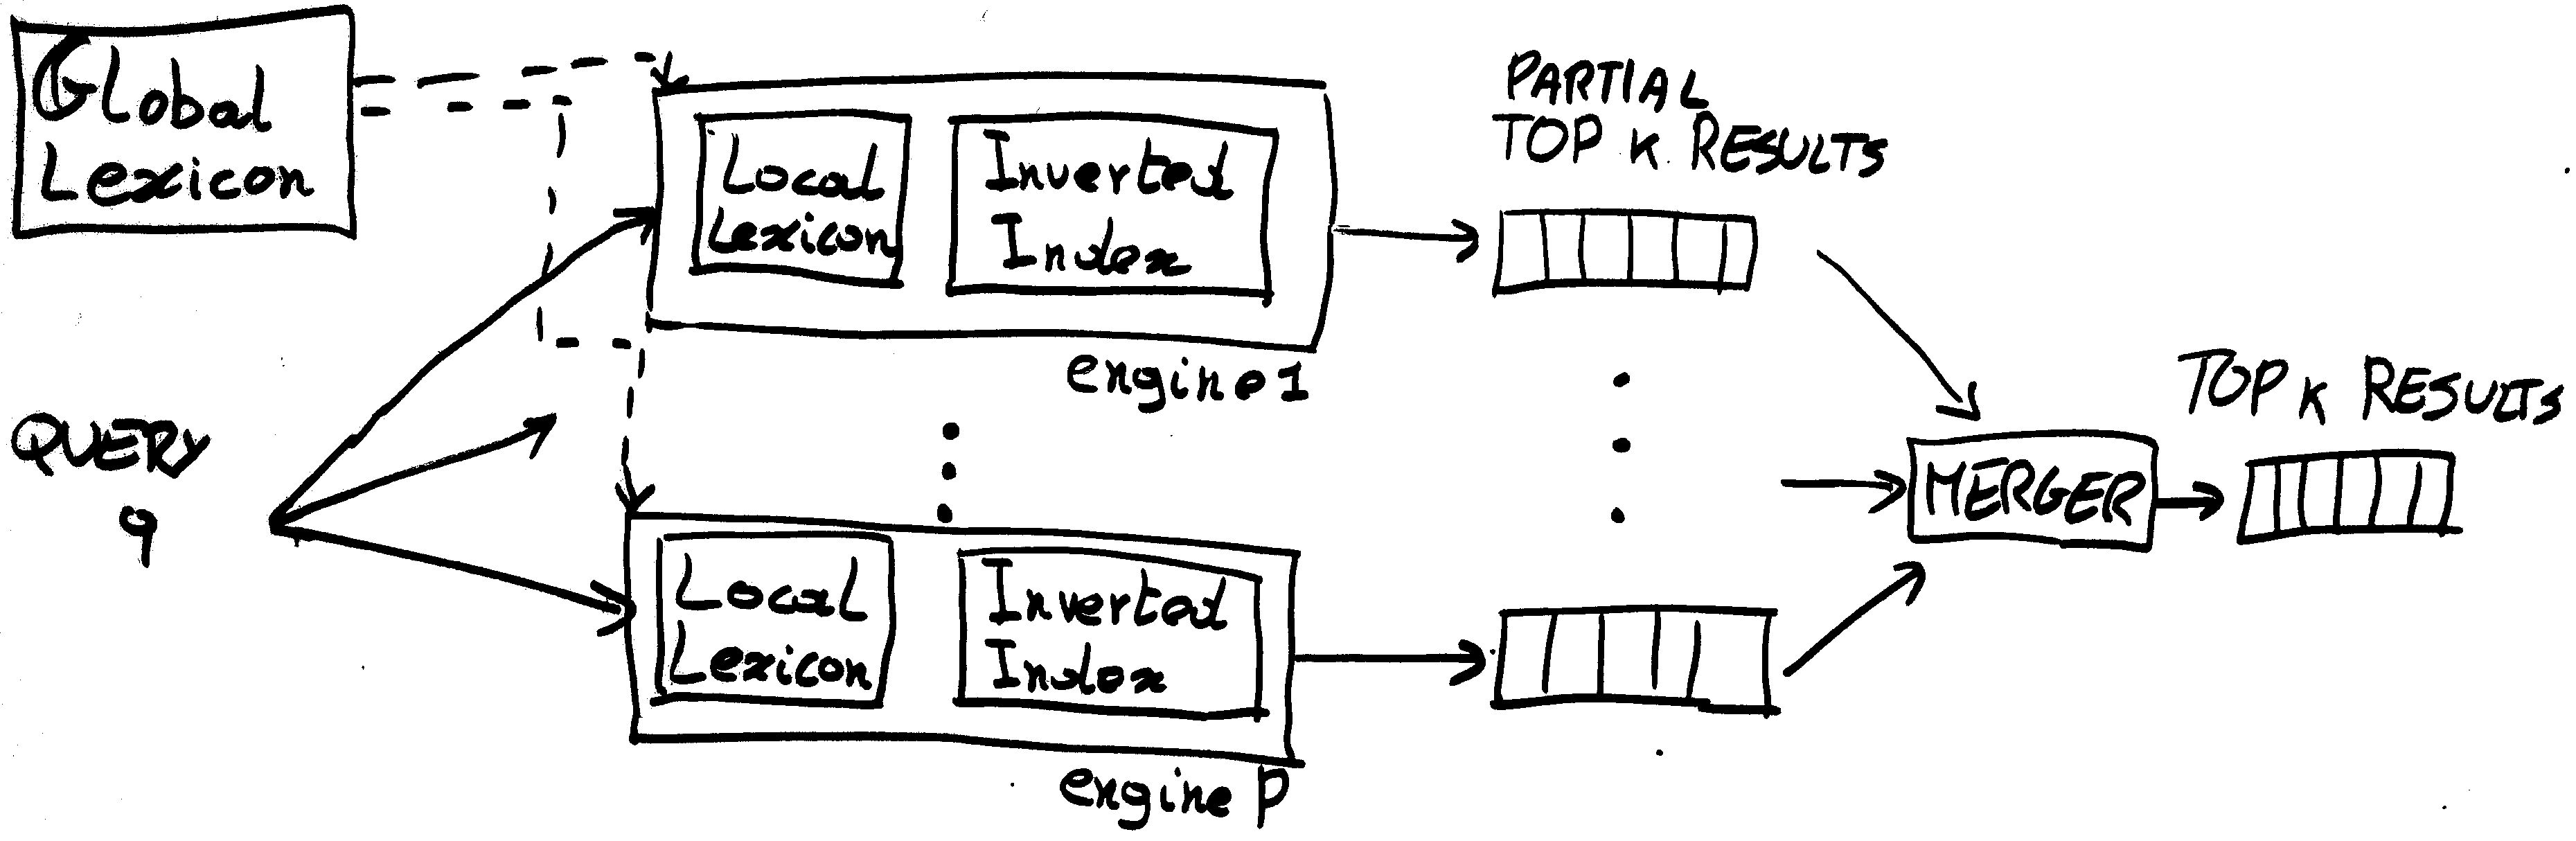
\includegraphics[width=0.95\linewidth]{assets/map_reduce}
	\caption{Not pictured: each partition has its own document index}
	\label{fig:mapreduce}
\end{figure}


\section{Indices}

\paragraph{}
The inverted indices are relatively straight-forward, they consist of two files; one for the documents' ids and the other for the associated term's frequencies, the former is encoded using \textit{variable bytes} while the latter in \textit{unary code}. The pointers to each region of the index --- that is the index's entry relative to a certain term --- are stored in the lexicon as explained in section \ref{subsection:lexicon-data}.

\section{Lexica}

Since we're partitioning the dataset by document, to improve its parallelizability we make use of a local lexicon for each partition as well as a global lexicon used to store shared information.

\subsection{Disk Map}

To store the lexica it is necessary to use a disk-based data structure that
allows the program to quickly and efficiently seek the datum associated to a
particular key, that is an index term. To achieve this we make use of following:

\begin{itemize}
	\item to reduce disk seek time, the terms' data are compressed with
	\textit{integer compression} and the terms themselves with \textit{prefix compression}
	
	\item to minimize disk accesses, the terms are ordered lexicographically
	and partitioned in pages of the same size of the disk's page
	
	\item terms at the beginning of each page are stored in a separated array that fits in system memory, to quickly locate --- through \textit{binary search} or a \textit{trie visit} --- in which page a given term is located
\end{itemize}

\paragraph{Structure}
Let us call $|B|$ the size of a disk page, $|T|$ the maximum length off all terms stored, $m$ the maximum number of key-value pairs stored in a page, $k$ the number of pages used to store them all, $s_1 > s_2 > s_3 > \dots$ the terms to store and $d_1, d_2, d_3, \dots$ their data; and $s_{b_1} > s_{b_2} > \dots > s_{b_k}$ the terms that appear at the start of each page.

The following picture shows how our data are organized at high level

\begin{figure}[H]
	\centering
	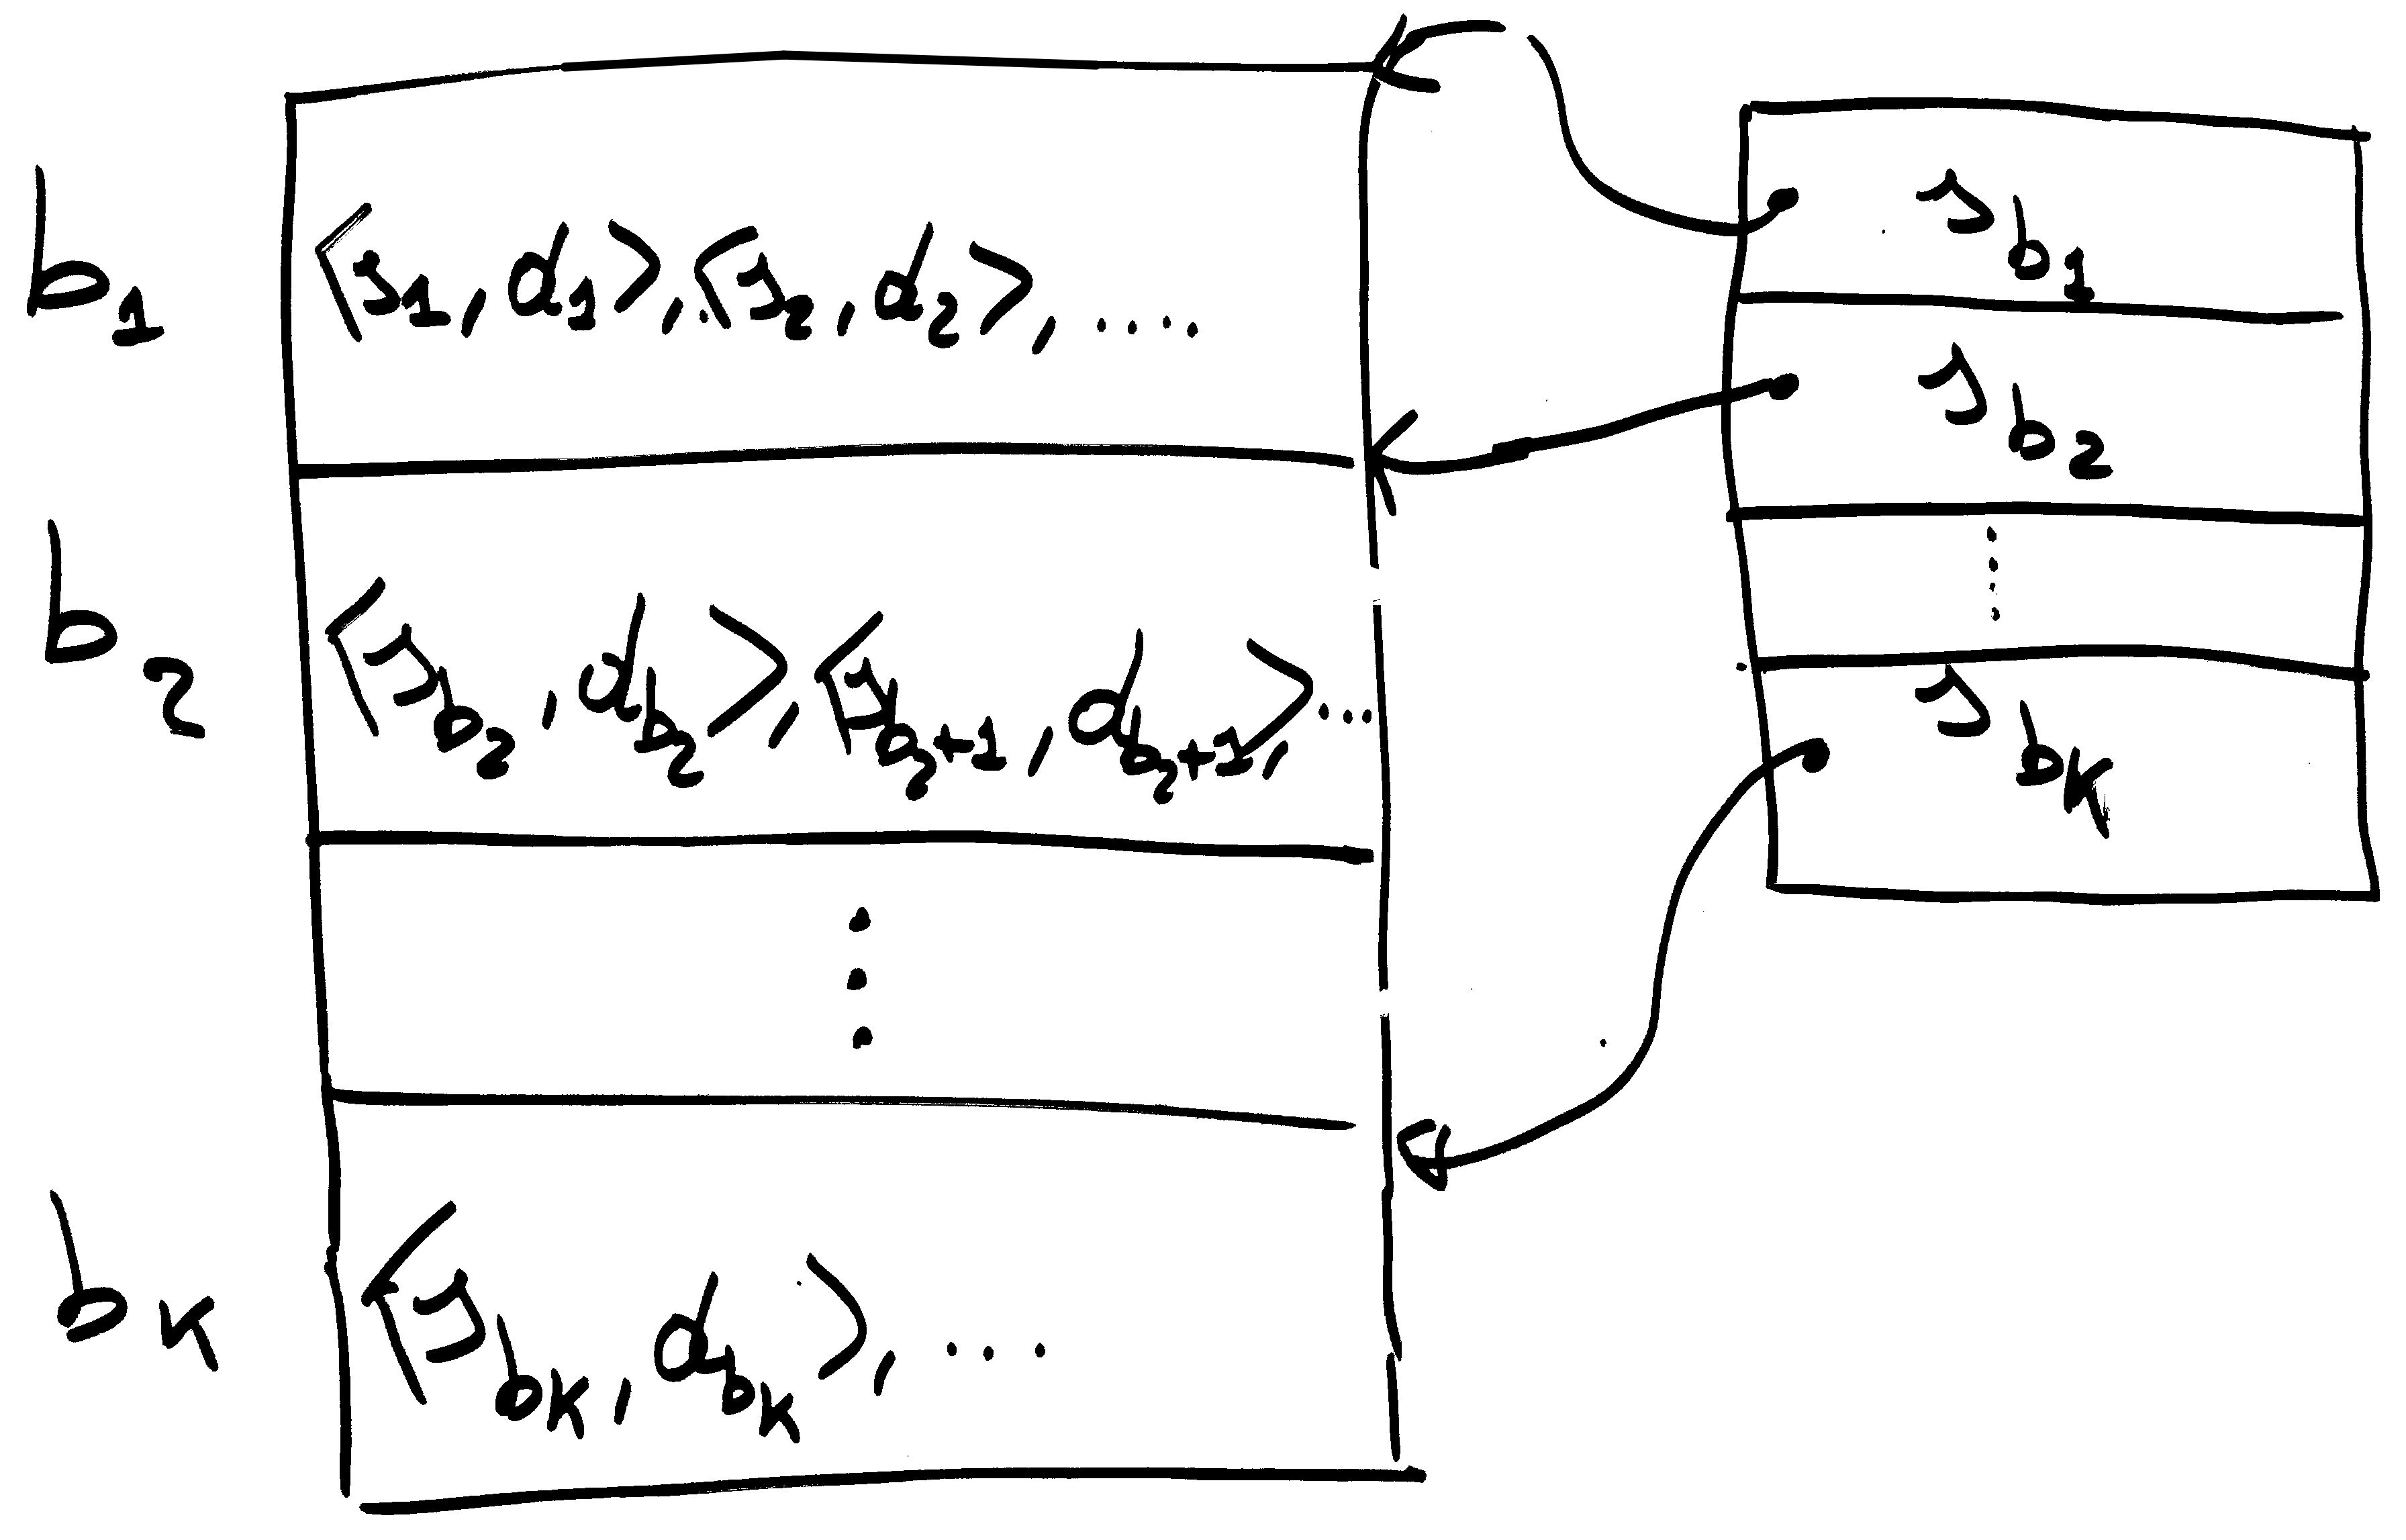
\includegraphics[width=0.6\linewidth]{assets/disk_map_base}
	\caption[]{Data organization}
	\label{fig:diskmapbase}
\end{figure}

In the real implementation, the pages' term heads $s_{b_i}$ are only stored in the look-up table, the data $d_i$ are compressed using \textit{variable bytes} and the other strings $s_j$ are compressed by cutting the common prefix they've with the page's head, so a generic key-value pair is more like:
$\left<	\left< p(s_{b_i}, s_j), {s'}_j \right>, c(d_j)	\right>$; where $p()$ is the length of the common prefix, $ {s'}_j$ is the string without the common prefix, and $c(d_j)$ is the compressed datum. The prefix's length is stored on a eight bit unsigned number, thus allowing for a maximum term's length of 255 bytes.

\paragraph{Complexity}
For simplicity's sake our implementation makes use of binary search to find in which page a term is stored and a linear scan to find it in the page, giving us a time complexity of 
$O\left(	|T|\cdot\log(k) + m	\right)$,
a space complexity, with regard to system memory, of
$O\left(	|T|\cdot k	\right)$
--- since we only have to keep the heads in memory --- and an I/O complexity of
$O\left(	1	\right)$, assuming all pages' heads fit in memory.

\subsection{Data}
\label{subsection:lexicon-data}

\paragraph{Local lexica}
Each local lexicon stores the terms' information as \texttt{LexiconValue} during the first pass and then as \texttt{SigmaLexiconValue} in the second pass, when the upper bounds are computed and the skipping lists built.

Both structures store the number of docs in which such term appears and pointers to the compressed term frequencies and documents' ids. The latter structure also contains the skipping list and the upper bounds for \textit{TFIDF} and \textit{BM25}.

\paragraph{Global lexicon}
The only global lexicon just stores the total number of documents each term appear in, this is necessary to correctly compute the \textit{IDF} term.

\begin{figure}[H]
	\centering
	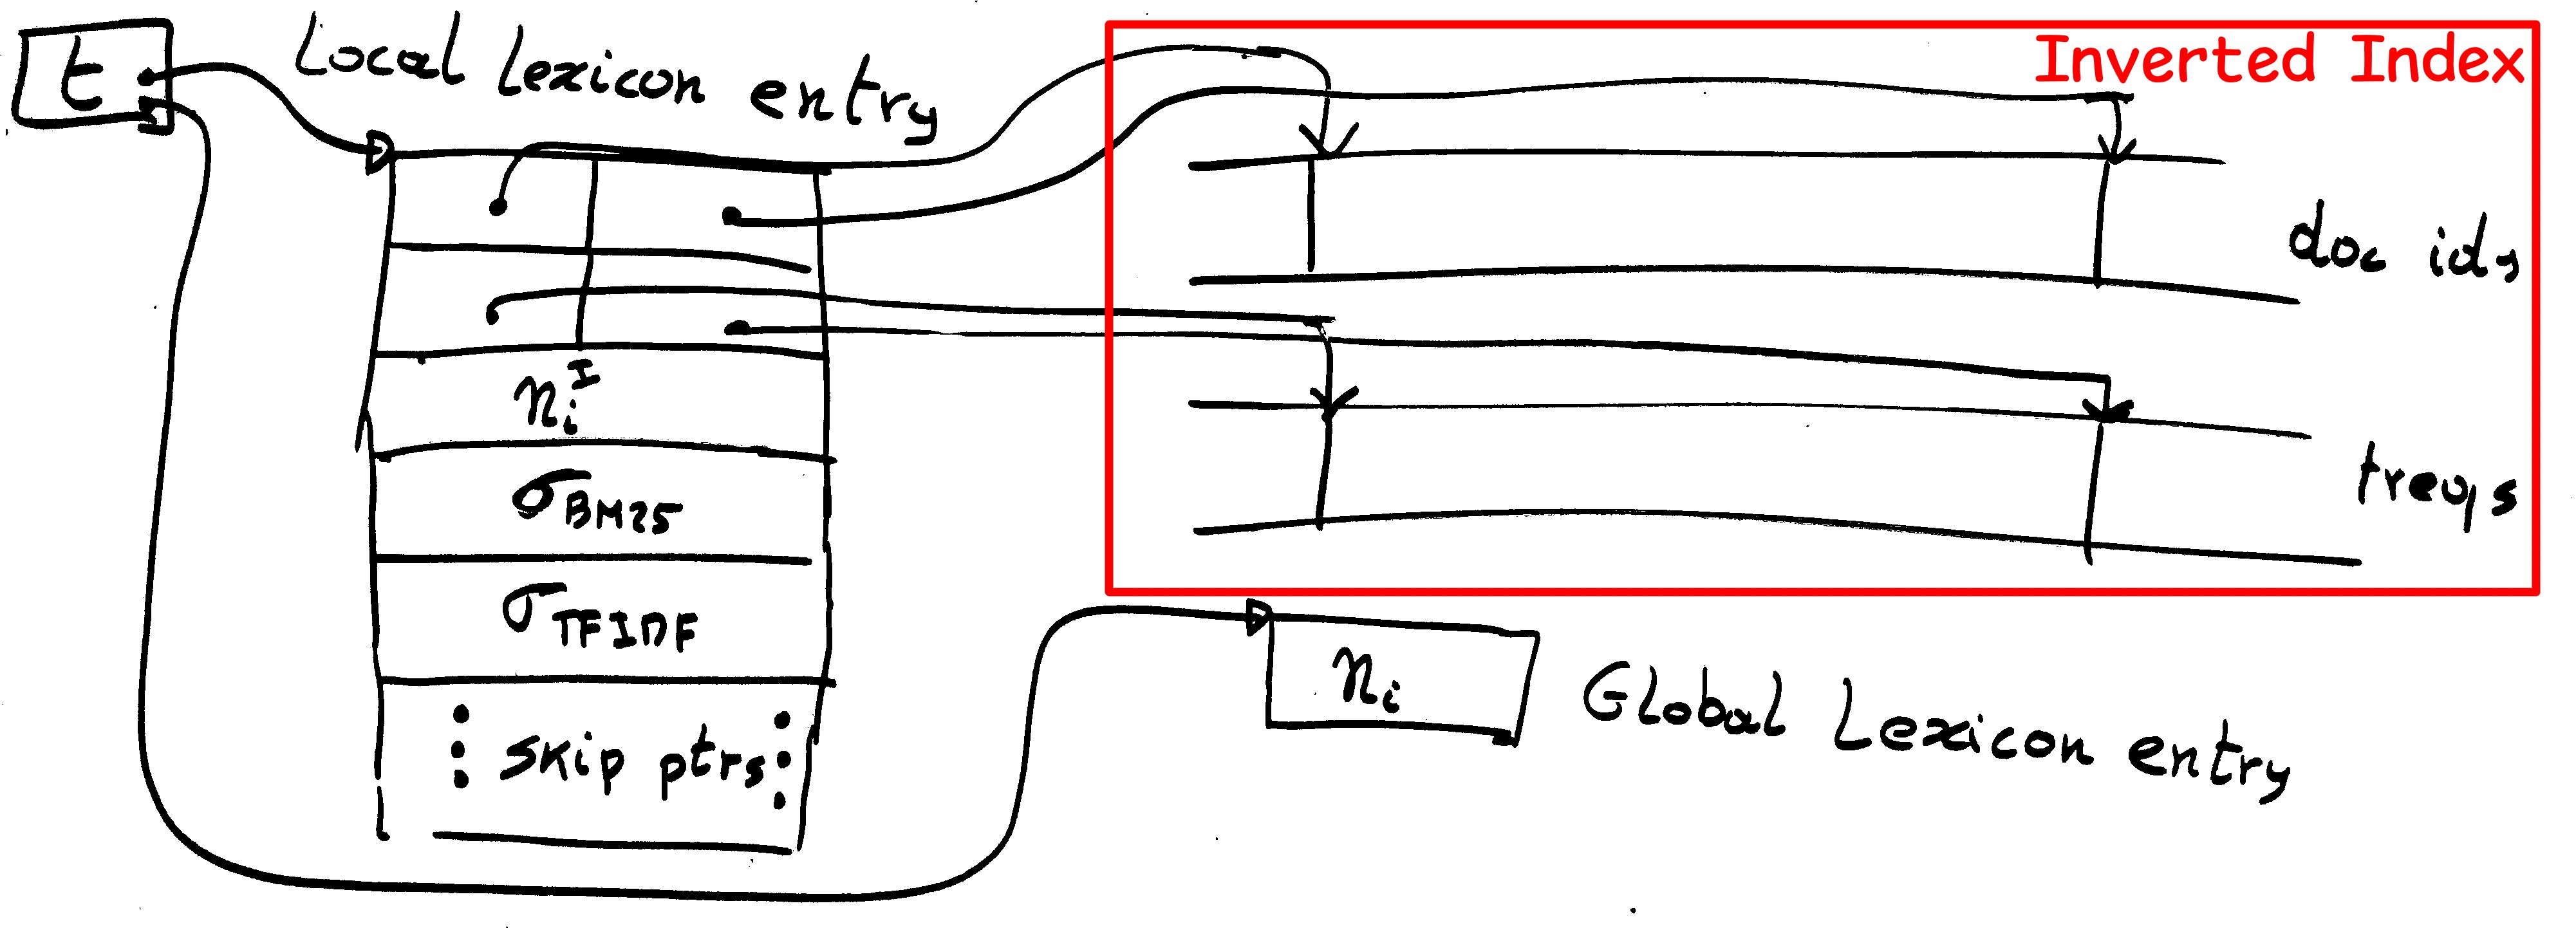
\includegraphics[width=0.9\linewidth]{assets/lexica}
	\caption{Overall representation of the lexica's data. ${n'}_i$ is an addendum that's used during the building phase to compute the total $n_i$}
	\label{fig:lexica}
\end{figure}

\section{Document Index}

\paragraph{}
The document index is the most straight-forward data structure, all entries have the same length --- that is sixteen bytes --- allowing access to the document's information in constant time $O(1)$ and with a single I/O read; this is crucial as access to the document's length is continuously performed when ranking with BM25 et similia.

\paragraph{docno}
To access the document's number we have to pay another I/O access, but that's not very important as the this access is only done once, at the end of the query solution algorithm.

\begin{figure}[h]
	\centering
	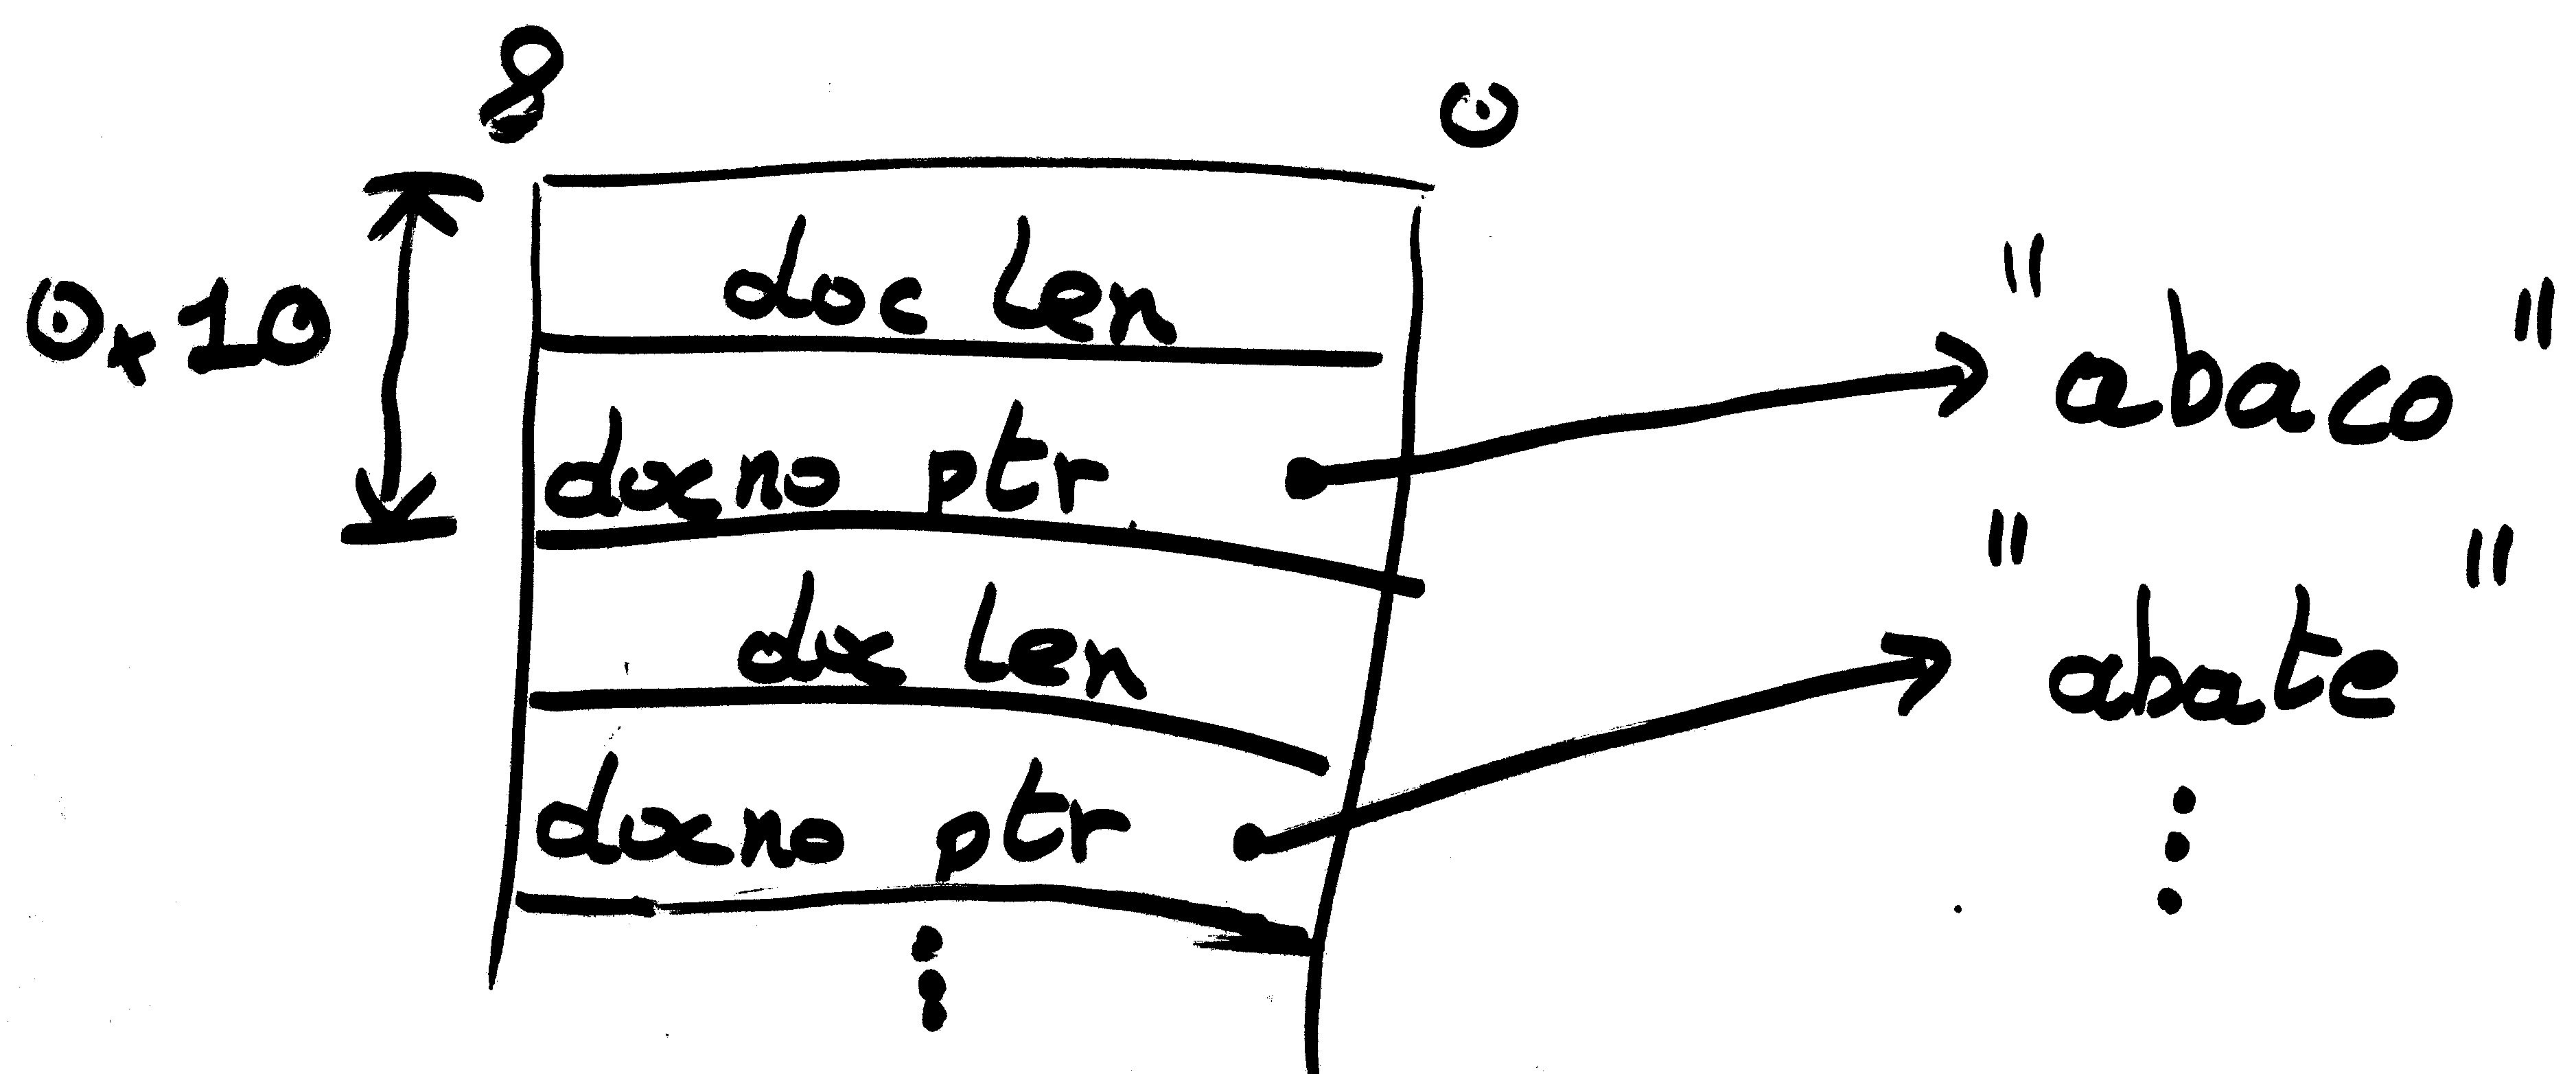
\includegraphics[width=0.7\linewidth]{assets/document_index}
	\caption{The document index, strings are stored at the end of the same file}
	\label{fig:documentindex}
\end{figure}

\section{Caches}

\paragraph{}
For simplicity's sake, we do not use caches, even though they might've improved performance; however, since we memory-map all files --- through the use of the POSIX system call \texttt{mmap()}, --- we have some sort of \textit{implicit cache} handled directly by the Kernel, as the most used disk pages are likely to be kept in system memory as the process progresses in its execution.

This is particularly advantageous when access the lexica and the document indices; especially for the latter, we can truly exploit this mechanism to obtain real $O(1)$ access times.

